% !TeX spellcheck = en_US
\documentclass[11pt,xcolor=dvipsnames,professionalfonts]{beamer}

% Pakete
\usepackage[utf8]{inputenc}
\usepackage[english]{babel}

% AMS Pakete
\usepackage{amsmath}
\usepackage{amsfonts}
\usepackage{amssymb}
\usepackage{mathtools}

% Text tools
\usepackage{textcomp}

% Einheiten
\usepackage{siunitx}
\sisetup{
	separate-uncertainty
}

% Grafiken
\usepackage{graphicx}
\usepackage{booktabs}
\usepackage{multirow}
\usepackage{caption}
\usepackage{subcaption}
\setbeamerfont{caption}{size=\footnotesize}
\setbeamertemplate{caption}{\raggedright\insertcaption\par}
\usepackage[percent]{overpic}

% Theme
\usetheme{Boadilla}
\usecolortheme{rose}
\useoutertheme{infolines}
\useinnertheme{rectangles}
\setbeamertemplate{itemize subitem}[triangle]

\usefonttheme[onlymath]{serif}

% [num] Zitationen
\setbeamertemplate{bibliography item}[text]

% Navigationsleiste ausschalten
\beamertemplatenavigationsymbolsempty

\author[Christian Bespin \& Christopher Deutsch]
{Christian Bespin \& Christopher Deutsch}

\title
{Analysis of $\mathrm{Z}^0$ Decays}

\subtitle
{}
%\logo{}

\institute[]
{Advanced Laboratory Course\\ Summer Term 16}

\date{May 30, 2016}

%\setbeamercovered{transparent}
%\setbeamertemplate{navigation symbols}{}

\newcommand{\beginbackup}{
	\newcounter{framenumbervorappendix}
	\setcounter{framenumbervorappendix}{\value{framenumber}}
}
\newcommand{\backupend}{
	\addtocounter{framenumbervorappendix}{-\value{framenumber}}
	\addtocounter{framenumber}{\value{framenumbervorappendix}} 
}

\begin{document}
\maketitle


\begin{frame}{Outline}
	\tableofcontents
\end{frame}

\section{Introduction}
\begin{frame}{Introduction}
		\begin{itemize}
			\setlength\itemsep{1em}
			\item Data from OPAL experiment at LEP provided
			\item Measure properties of $\mathrm{Z}^0$ boson: mass, decay width
			\item Analyze each decay channel separately
			\item Use results to determine Weinberg angle and number of light neutrino generations
			\item Show lepton universality
		\end{itemize}
\end{frame}

\section{Theoretical Background}
\begin{frame}{$\mathrm{Z}^0$ Boson}
	\begin{itemize}
		\item Mass $M_\mathrm{Z} = \SI{91.1876 +- 0.0021}{GeV}$
		\item Decay width $\Gamma_\mathrm{Z} = \SI{2.4952 +- 0.0023}{GeV}$\footnote{Particle Data Group, \emph{The Review of Particle Physics} 2014 and 2015 update}
		\item Can decay into all leptons and quarks (except top quark)
		\item In general all processes possible with photon propagator
	\end{itemize}
	\begin{figure}[htb]
		\centering
		\begin{subfigure}{.28\textwidth}
			\centering
			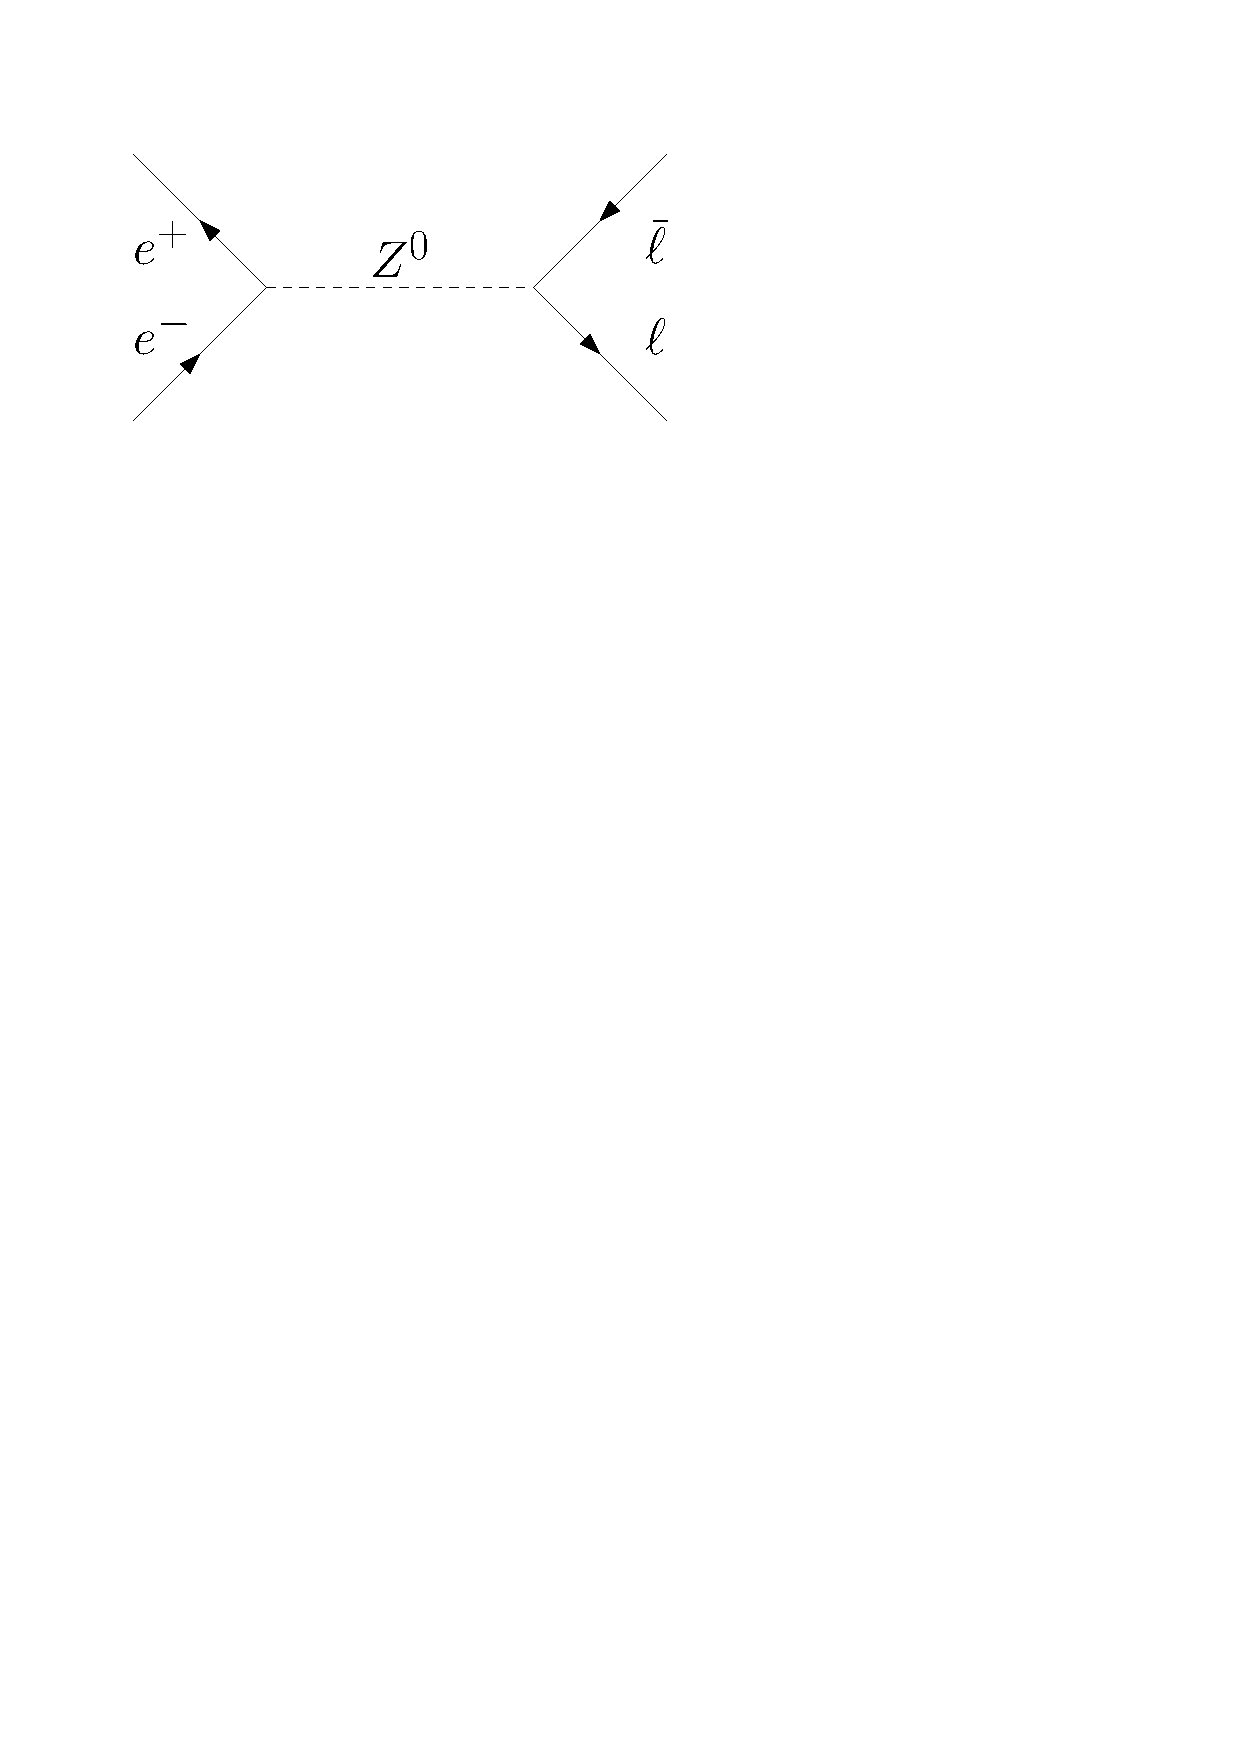
\includegraphics[width=.8\textwidth]{./figures/theory/feynman/ll}
		\end{subfigure}
		\begin{subfigure}{.28\textwidth}
			\centering
			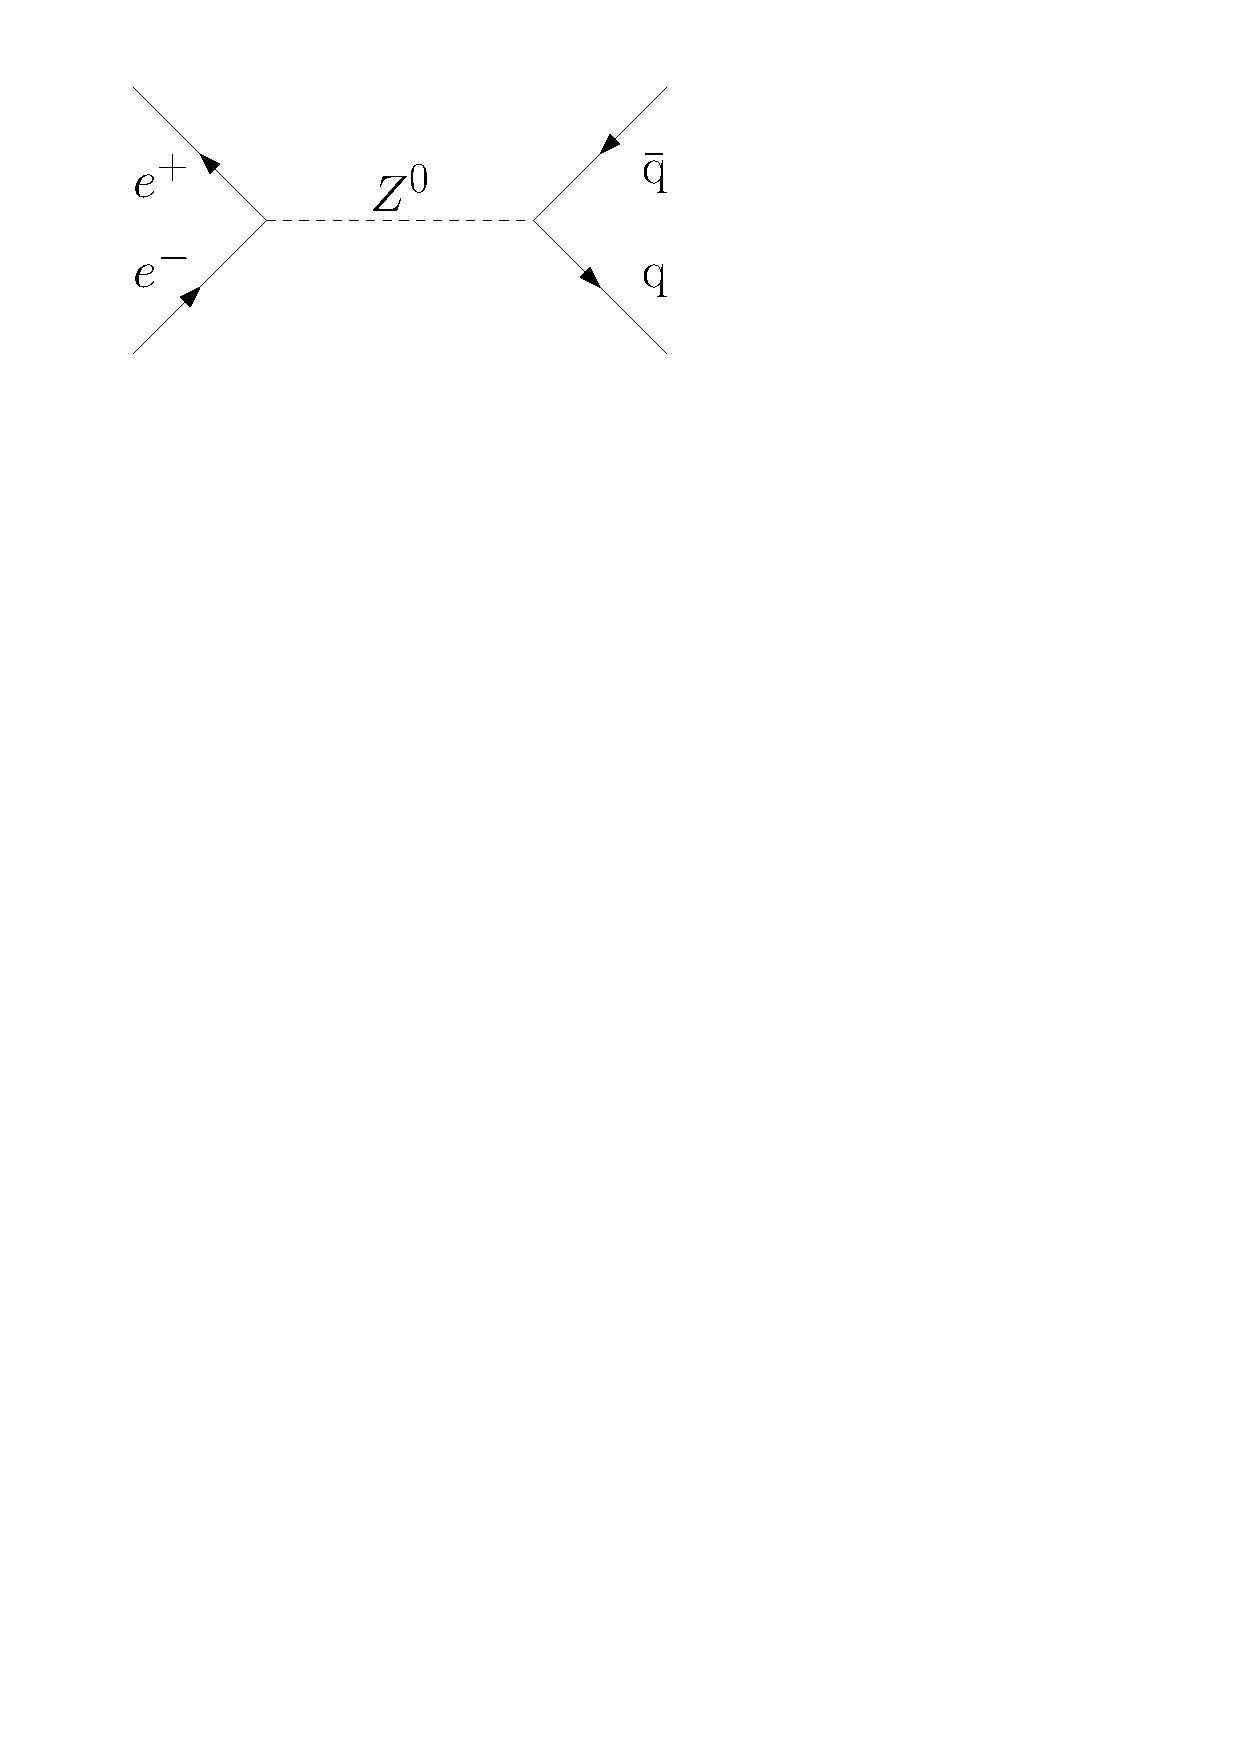
\includegraphics[width=.8\textwidth]{./figures/theory/feynman/qq}
		\end{subfigure}
		\begin{subfigure}{.28\textwidth}
			\centering
			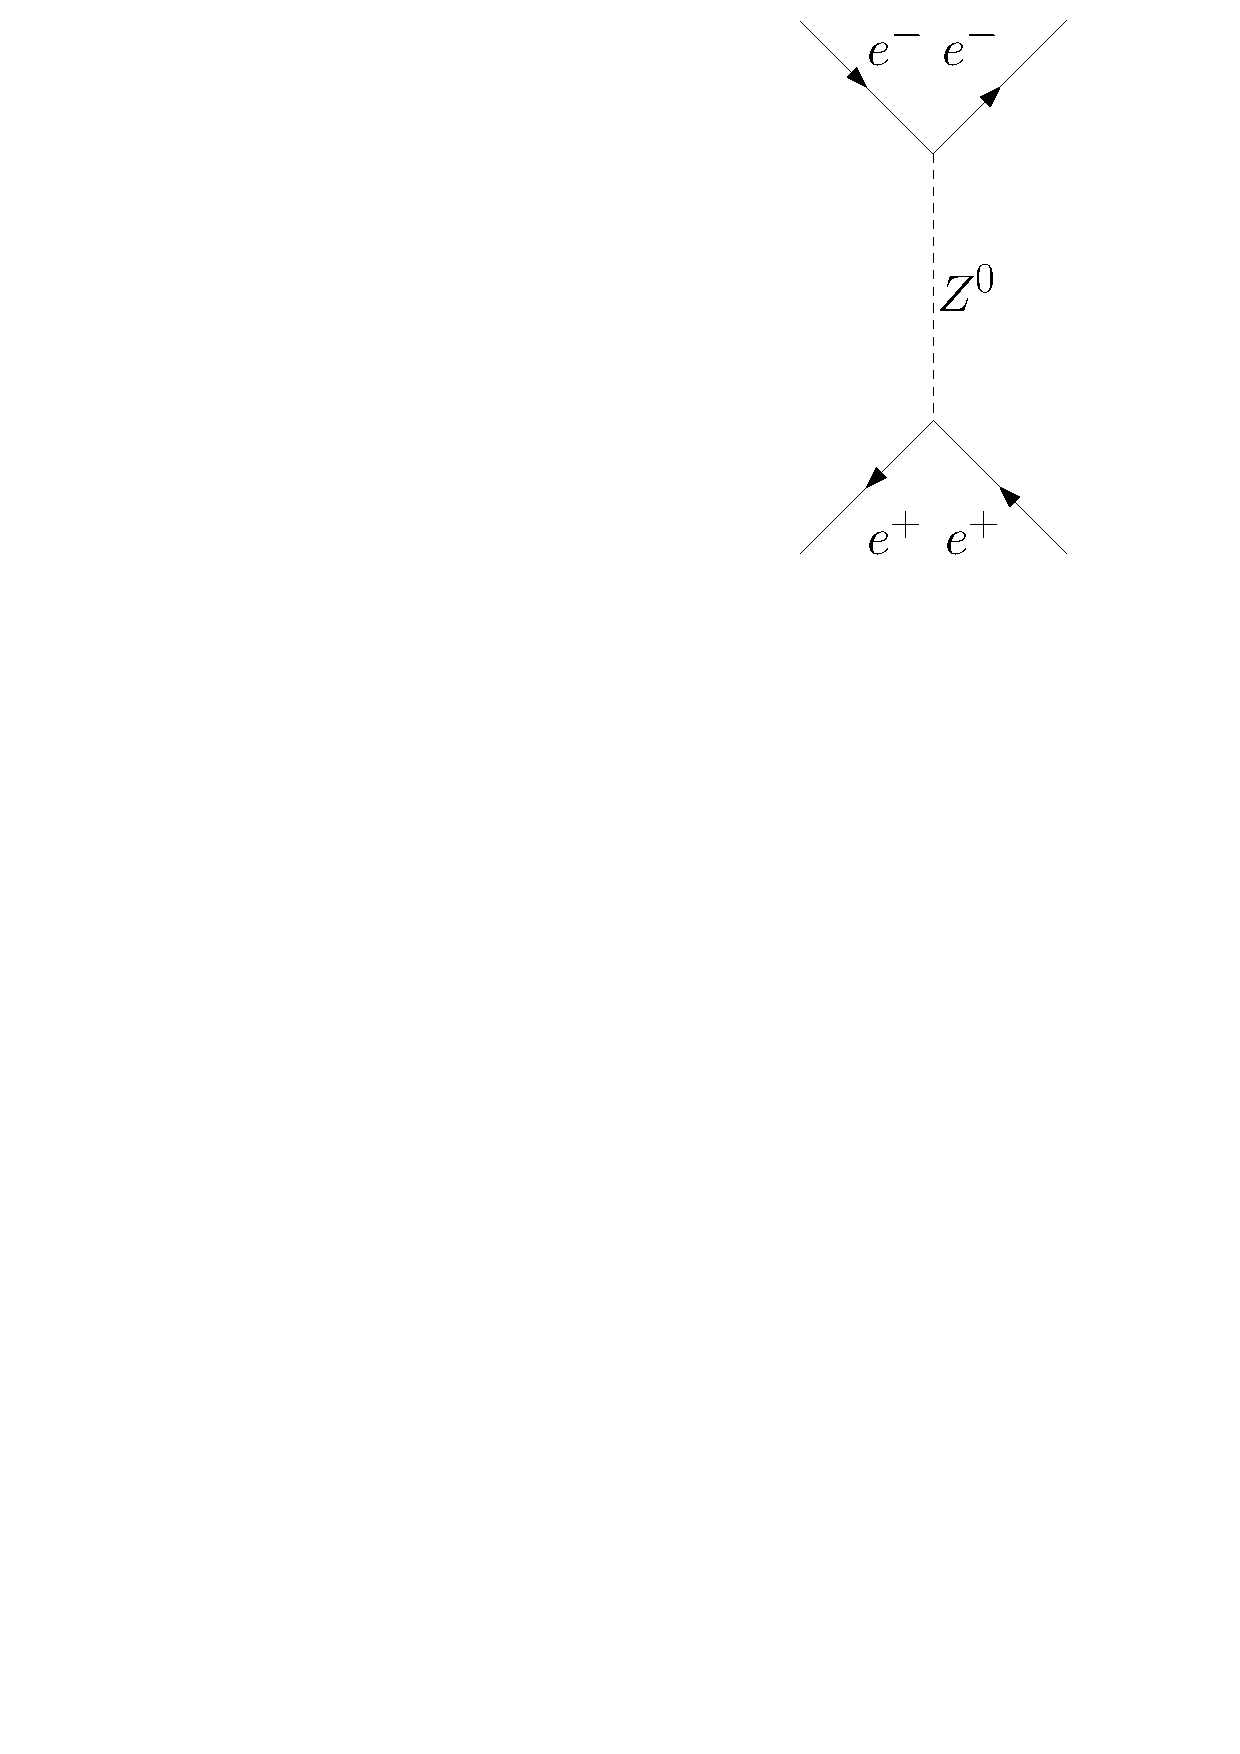
\includegraphics[width=.8\textwidth]{./figures/theory/feynman/ee_t}
		\end{subfigure}
	\end{figure}
\end{frame}

\begin{frame}{Theoretical Background}
	Angular dependence of differential cross section
	\begin{itemize}
		\item $e^+e^-\rightarrow e^+e^-$ possible in $s$- and $t$-channel
		\item In $s$-channel, $\frac{\mathrm{d}\sigma}{\mathrm{d}\Omega}\propto(1+\cos^2\theta)$, in $t$-channel $\frac{\mathrm{d}\sigma}{\mathrm{d}\Omega}\propto(1-\cos\theta)^{-2}$
		\item Differentiate between channels with cut on $\theta$
	\end{itemize}
	\vspace{.5em}
	\begin{columns}
		\column[c]{0.2\textwidth}
		\centering
		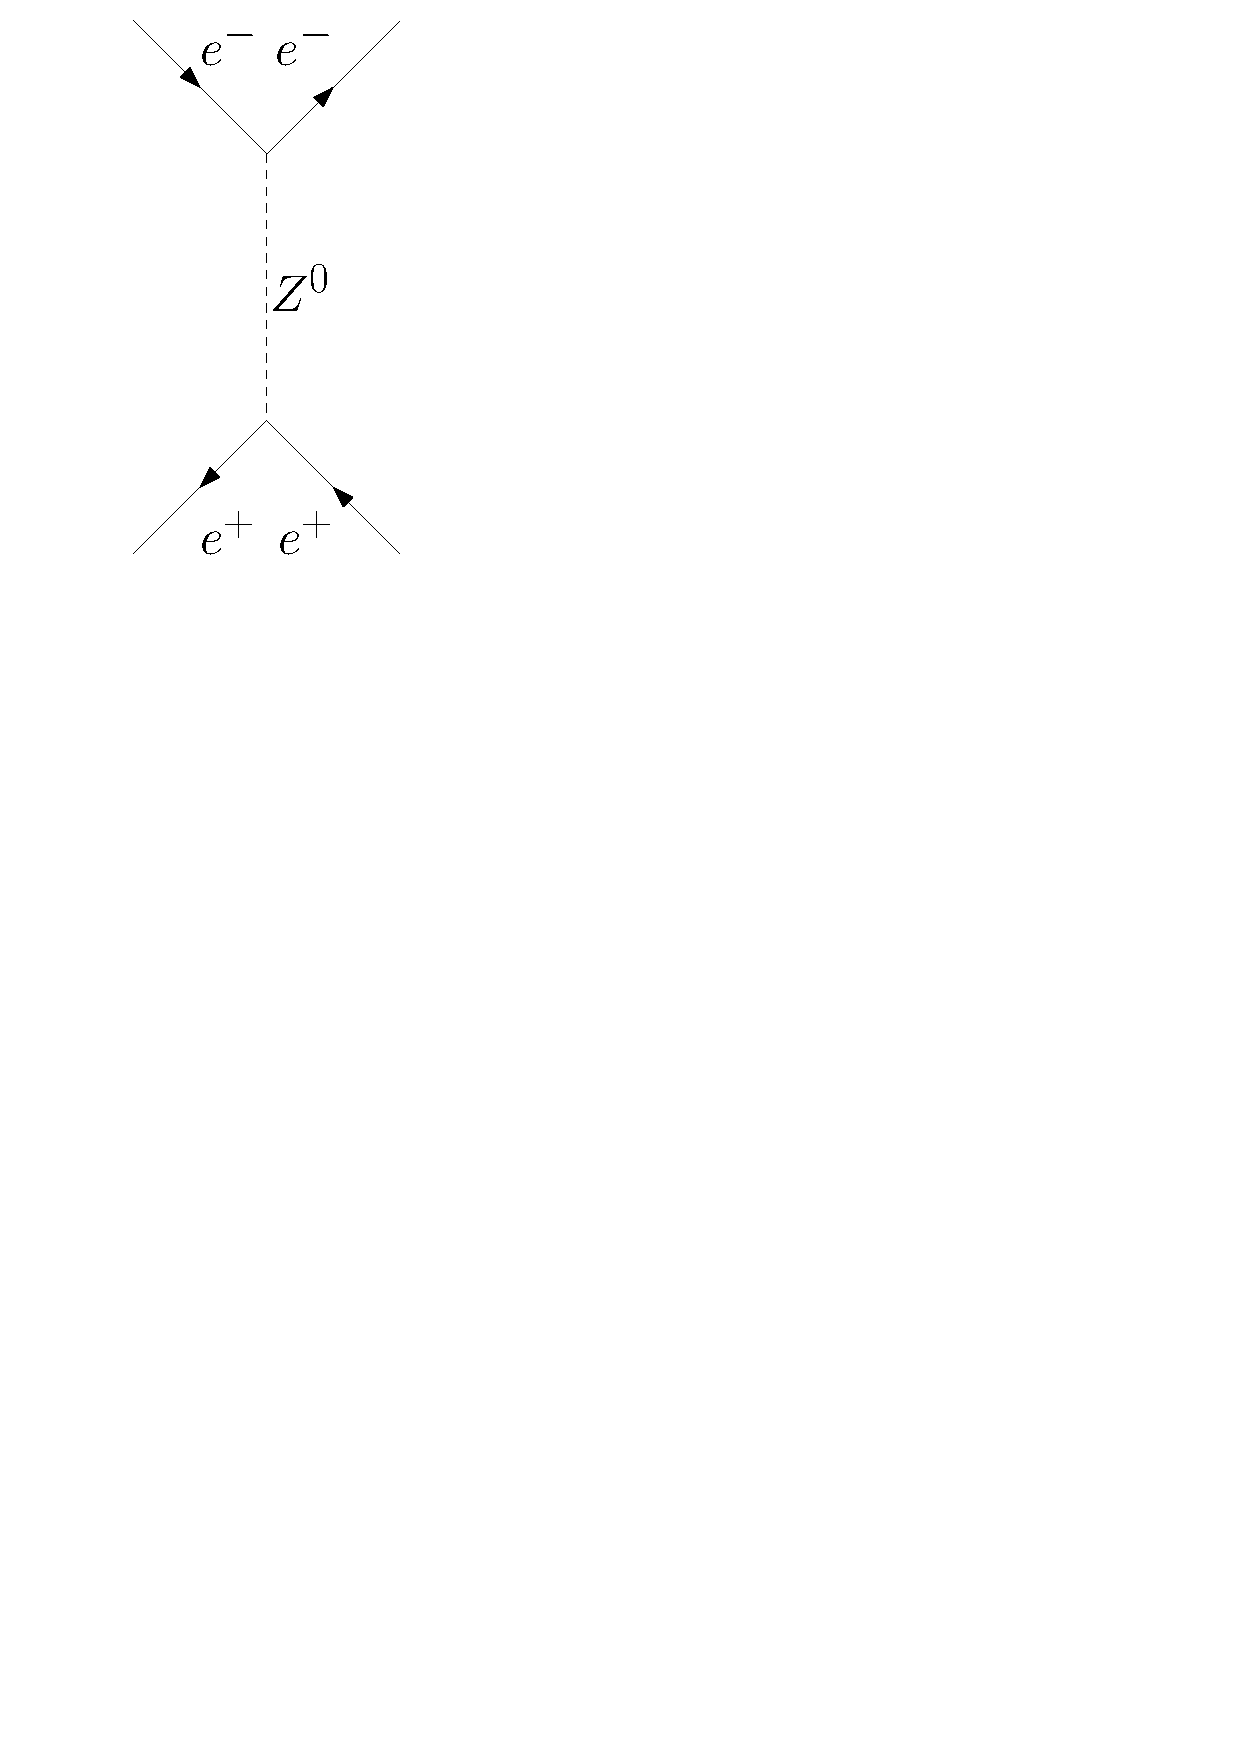
\includegraphics[width=.8\textwidth]{./figures/theory/feynman/t_z0}\\
		\footnotesize{rare}
		\column[c]{0.2\textwidth}
		\centering
		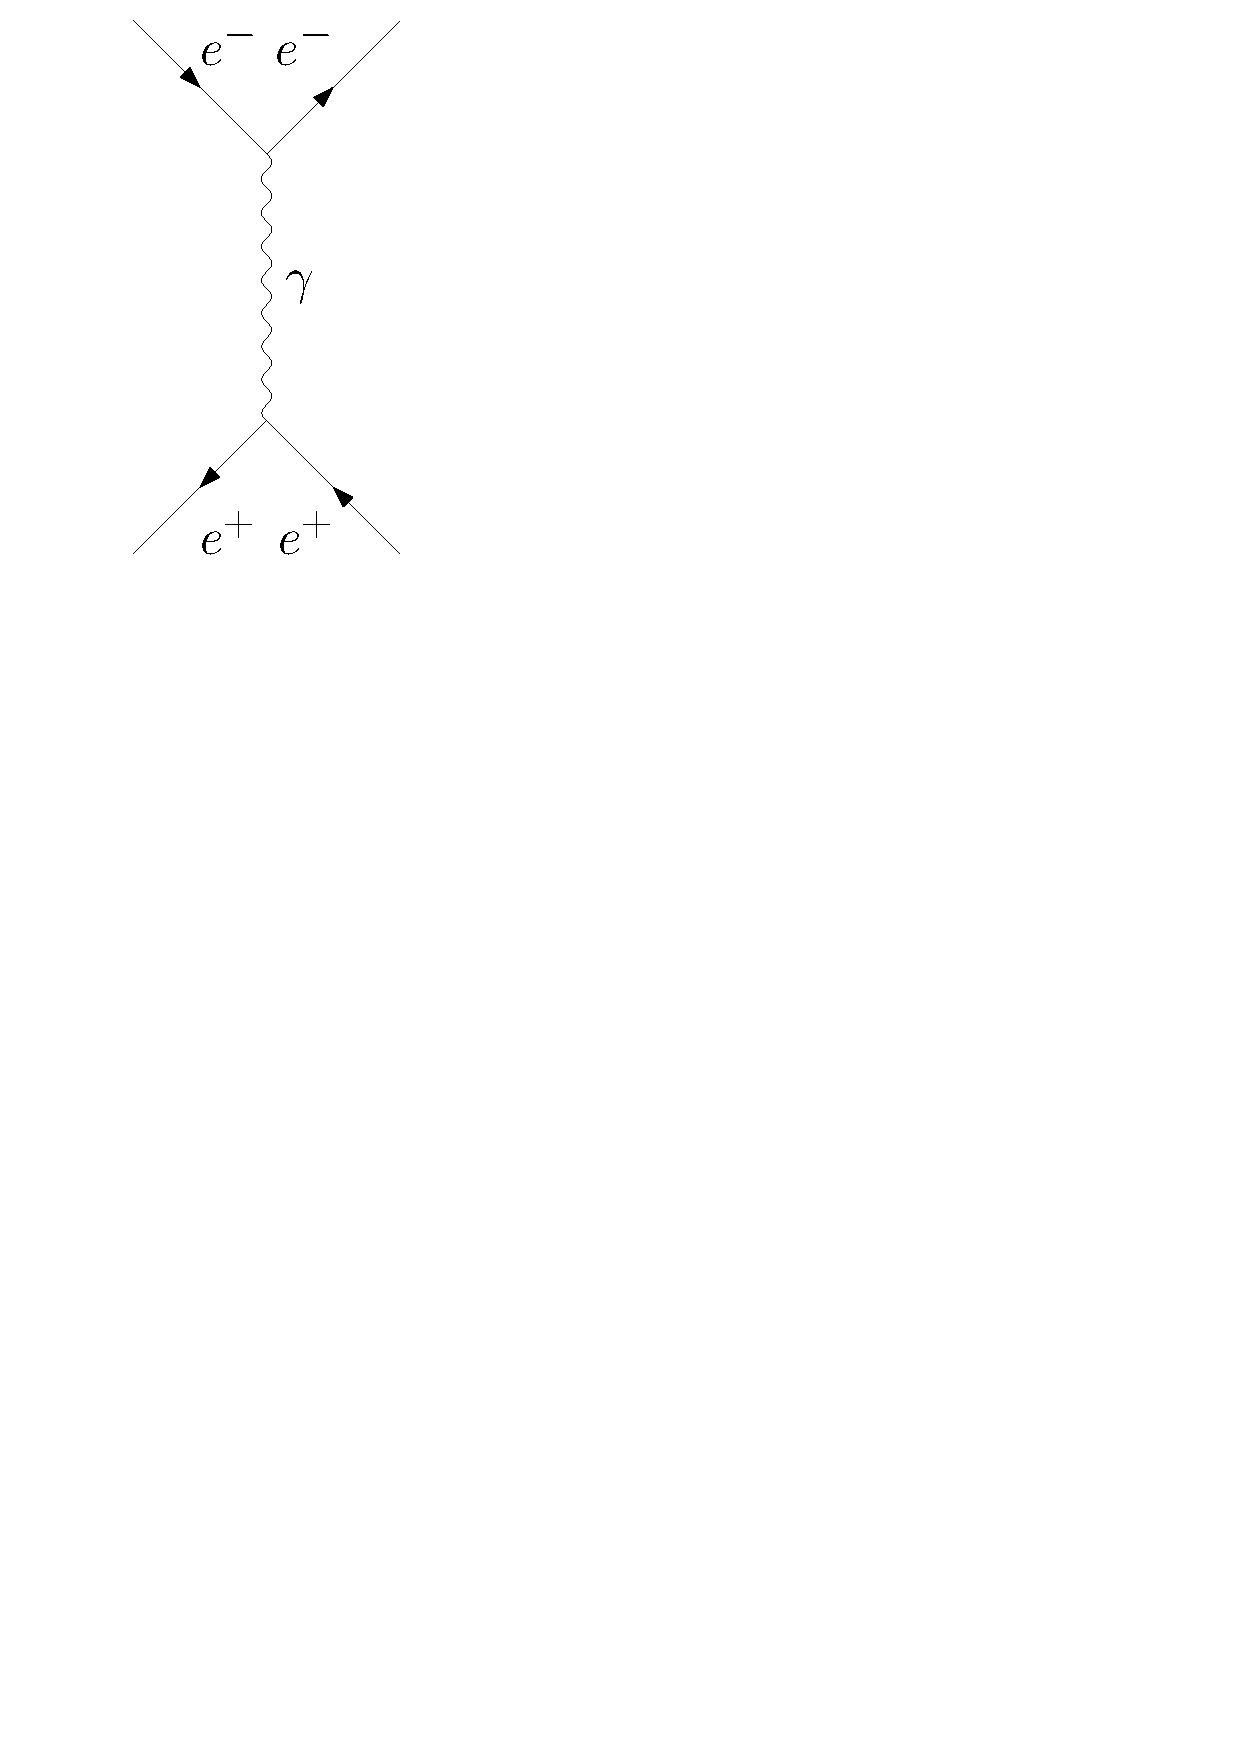
\includegraphics[width=.8\textwidth]{./figures/theory/feynman/t_gamma}\\
		\footnotesize{dominant}
		\column[c]{0.6\textwidth}
		\centering
		\vspace{3pt}
		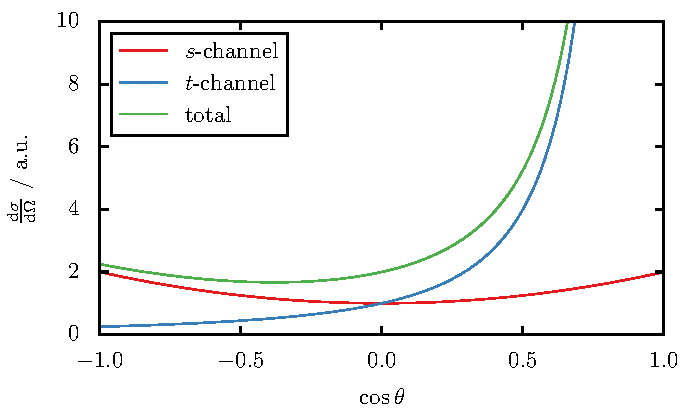
\includegraphics[width=\textwidth]{./talkfigs/pdf/s_t_channel}
	\end{columns}
\end{frame}

\begin{frame}{Theoretical Background}
	Weinberg angle
	\begin{itemize}
		\item Electroweak unification: combine electromagnetic and weak interaction
		\item Introduce weak isospin and weak hypercharge
		\item Gauge bosons of this gauge group are not observable
		\item Because of spontaneous symmetry breaking, combinations of two gauge bosons ($\mathrm{W}^3$ and $\mathrm{B}$) form observable $\mathrm{Z}^0$ and $\gamma$
	\end{itemize}
	\begin{align*}
		\begin{pmatrix}
		\gamma \\
		\mathrm{Z}^0
		\end{pmatrix} = 
		\begin{pmatrix}
		\cos\theta_\mathrm{W} & \sin\theta_\mathrm{W} \\
		-\sin\theta_\mathrm{W} & \cos\theta_\mathrm{W}
		\end{pmatrix}
		\begin{pmatrix}
		\mathrm{B} \\
		\mathrm{W}^3
		\end{pmatrix}
	\end{align*}
	\begin{itemize}
		\item Weak mixing angle (``Weinberg angle'') $\theta_\mathrm{W}$
		\item Describes relation between vector and axial-vector coupling
	\end{itemize}
\end{frame}

\begin{frame}{Theoretical Background}
	Forward-backward asymmetry
	\begin{itemize}
		\item In $e^+e^- \rightarrow f\bar{f}$, differential cross section different for forward and backward hemisphere $\rightarrow$ forward-backward asymmetry $A_\mathrm{FB}$
		\item $A_\mathrm{FB}$ for leptons and energies near the resonance ($v_\ell$, $a_\ell$ weak couplings)
		\begin{align*}
			A_\mathrm{FB}^{\mathrm{peak}}\approx 3\left(\frac{v_\ell}{a_\ell}\right)^2 = 3\left( 1 - 4 \sin^2\theta_\mathrm{W} \right)
		\end{align*}
		\item Measure $A_\mathrm{FB}$ in muon channel to determine Weinberg angle
		\begin{itemize}
			\item Clearest detector signature
		\end{itemize}
	\end{itemize}
\end{frame}

\section{Part I: Analysis of Event Displays}
\begin{frame}{Part I: Analysis of Event Displays}
	\begin{itemize}
		\setlength\itemsep{2.em}
		\item Understanding OPAL detector response
		\begin{itemize}
			\setlength\itemsep{0.5em}
			\item Looking at event displays with software \texttt{GROPE} (MC data)
			\item Classification of events by detector response
		\end{itemize}
		
		\item Derivation of preliminary cut selections
		\begin{itemize}
			\setlength\itemsep{0.5em}
			\item Analyze each decay channel separately
		\end{itemize}
	\end{itemize}
\end{frame}

\begin{frame}{OPAL detector response}
	\begin{columns}
		\column[c]{0.5\textwidth}
		Electrons:
		\begin{itemize}
			\setlength\itemsep{.5em}
			\item $e^+e^-$ pair (two charged tracks)
			\item Mostly back-to-back events
			\item Energy deposited in e.m. calorimeter
		\end{itemize}
		\column[c]{0.5\textwidth}
		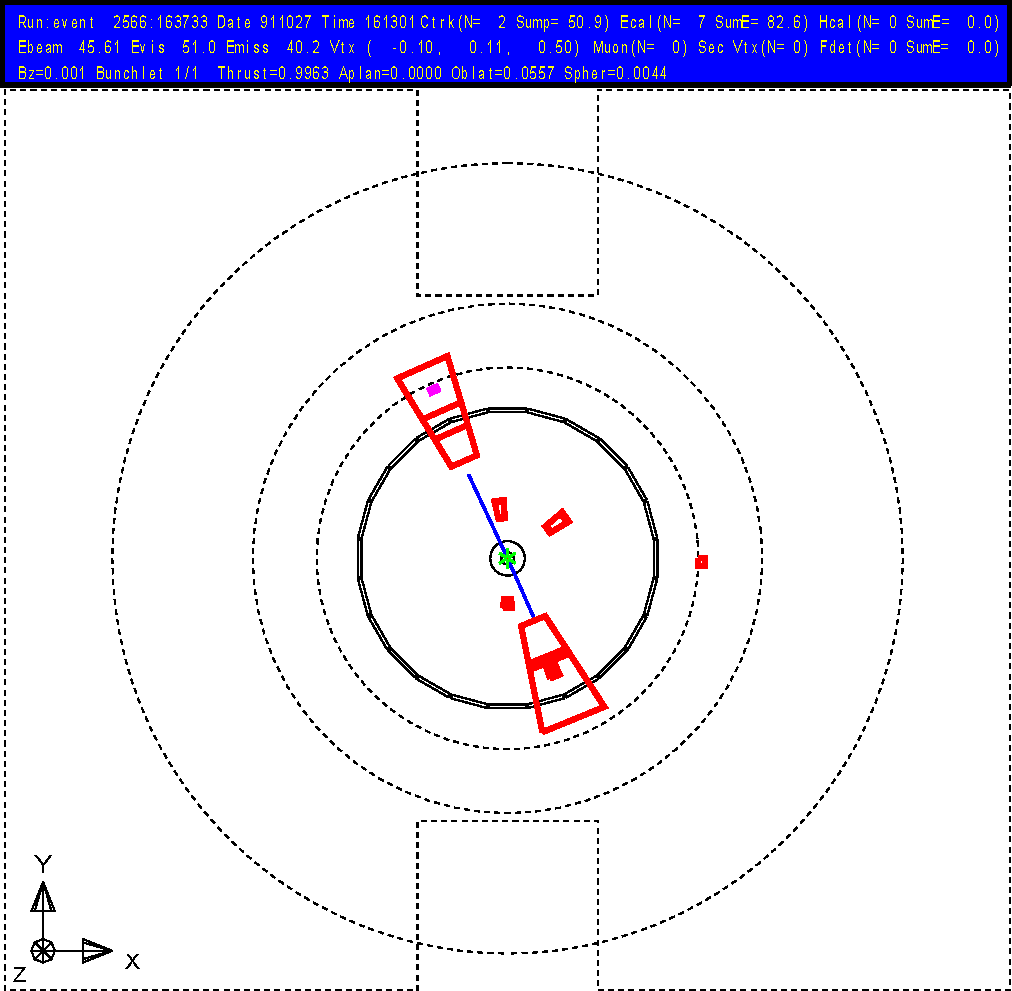
\includegraphics[width=1.0\textwidth]{./talkfigs/pdf/ee_02.pdf}

	\end{columns}
\end{frame}
\begin{frame}{OPAL detector response}
	\begin{columns}
		\column[c]{0.5\textwidth}
		Muons:
		\begin{itemize}
			\setlength\itemsep{.5em}
			\item $\mu^+\mu^-$ pair (two charged tracks)
			\item Back-to-back events
			\item No (small) energy deposited in calorimeters
			\item Signal in muon detector
		\end{itemize}
		\column[c]{0.5\textwidth}
		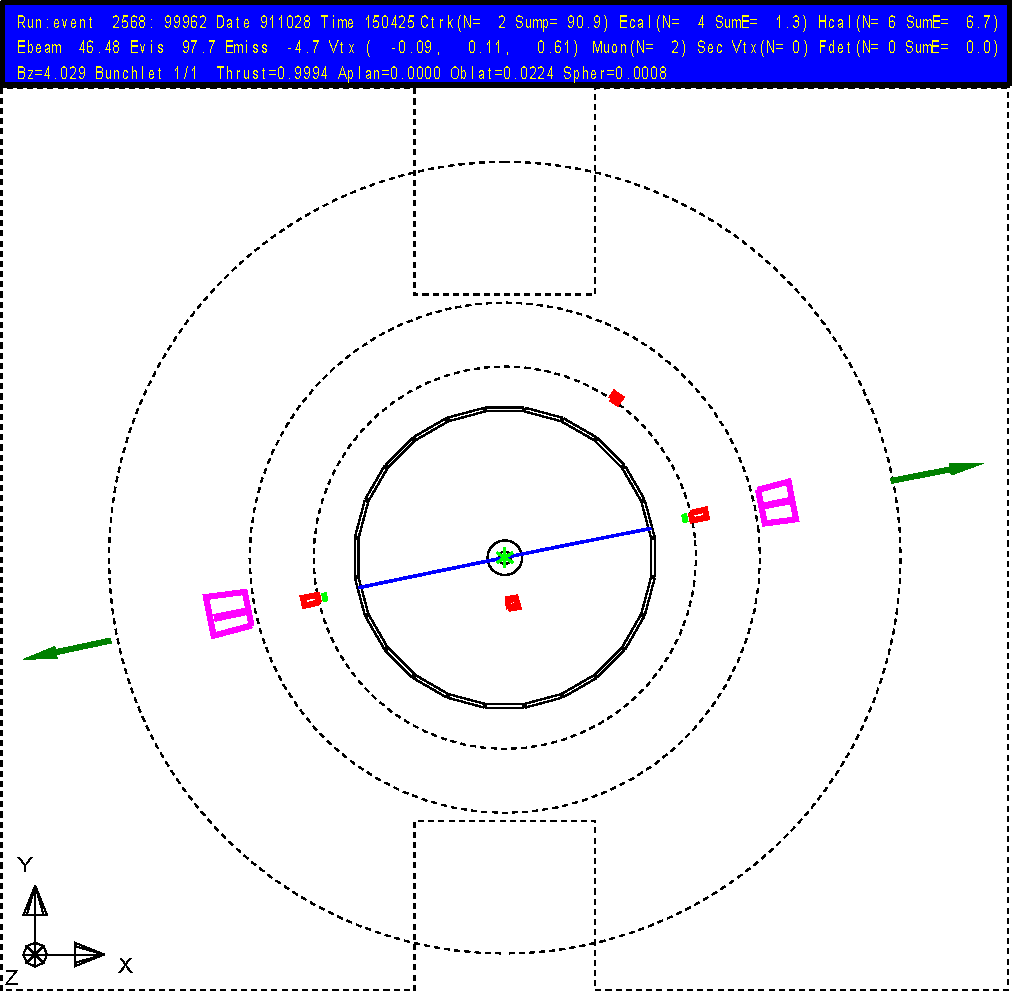
\includegraphics[width=1.0\textwidth]{./talkfigs/pdf/mm_02.pdf}
	\end{columns}
\end{frame}
\begin{frame}{OPAL detector response}
	\begin{columns}
		\column[c]{0.5\textwidth}
		Taus:
		\begin{itemize}
			\setlength\itemsep{.5em}
			\item $\tau^+\tau^-$ pair
			\item Short lifetime $\rightarrow$ decay into other particles before detection
			\item Detector response depends on decay product
			\item Event characterized by number of charged tracks (``prongs'')
		\end{itemize}
		\centering
		\begin{tabular}{lc}
			\toprule
			decay mode & br. ratio \\
			\midrule
			$\pi^\pm\pi^0\nu_\tau$ & \SI{25.52}{\percent} \\
			$e^\pm\nu_e\nu_\tau$ & \SI{17.83}{\percent} \\
			$\mu^\pm\nu_\mu\nu_\tau$ & \SI{17.41}{\percent} \\
			\bottomrule
		\end{tabular}
		\column[c]{0.5\textwidth}
		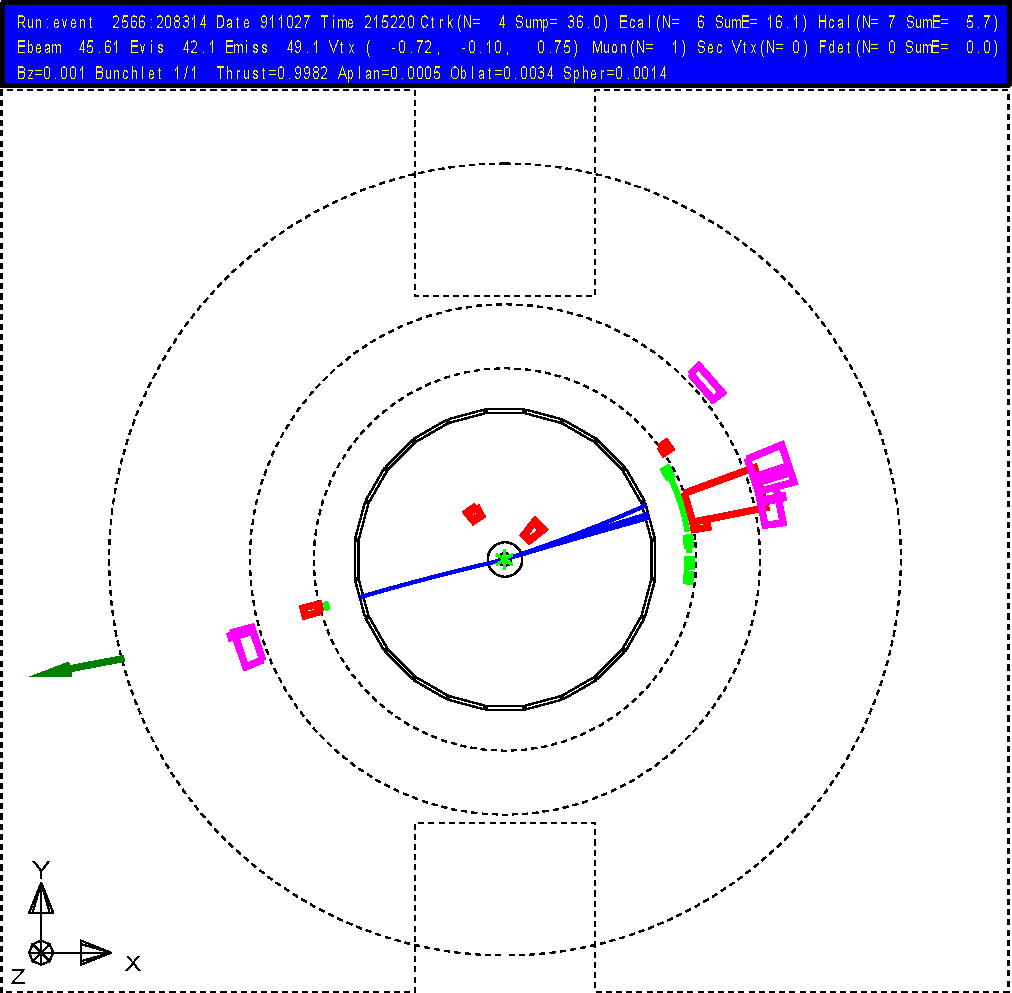
\includegraphics[width=1.0\textwidth]{./talkfigs/pdf/tt_05.pdf}
	\end{columns}
\end{frame}
\begin{frame}{OPAL detector response}
	\begin{columns}
		\column[c]{0.5\textwidth}
		Hadrons:
		\begin{itemize}
			\setlength\itemsep{.5em}
			\item Quark-antiquark pair initial decay products
			\item Due to confinement additional quarks created $\rightarrow$ formation of hadrons
			\item Deposit energy in hadron calorimeter
			\item Sometimes decay into leptons $\rightarrow$ signal in e.m. calorimeter
		\end{itemize}
		\column[c]{0.5\textwidth}
		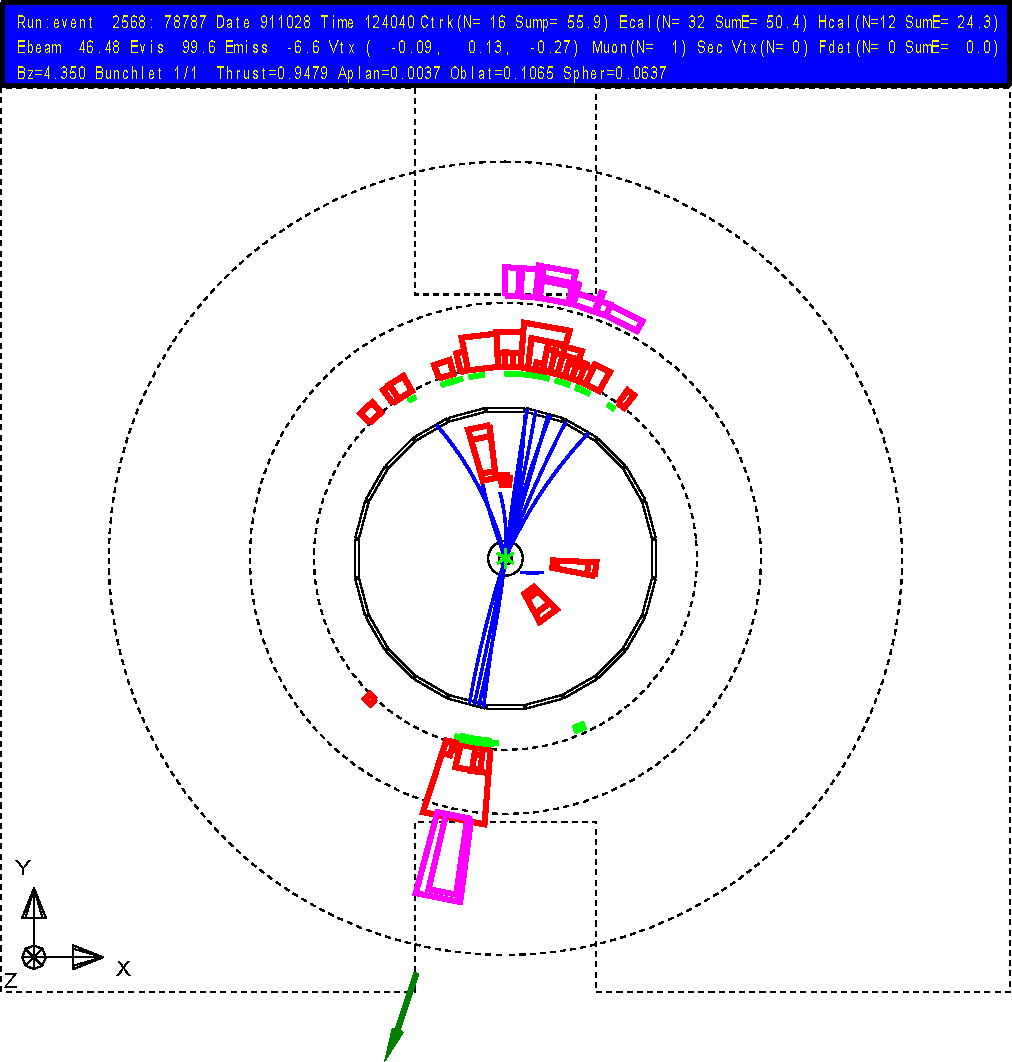
\includegraphics[width=1.0\textwidth]{./talkfigs/pdf/qq_04.pdf}
	\end{columns}
\end{frame}

\begin{frame}{Classification of Events}
	\begin{itemize}
		\setlength\itemsep{1em}
		\item Note measured quantities for every event:
		\begin{itemize}
			\setlength\itemsep{.5em}
			\item Number of charged tracks
			\item Total momentum of charged tracks
			\item Energies deposited in e.m. and hadron calorimeter
		\end{itemize}
		\item Plot distributions
		\item Formulate cuts to separate types of $\mathrm{Z}^0$ decays
	\end{itemize}
\end{frame}

\begin{frame}{Preliminary Cut Selections}
	\begin{columns}
		\column[c]{0.5\textwidth}
			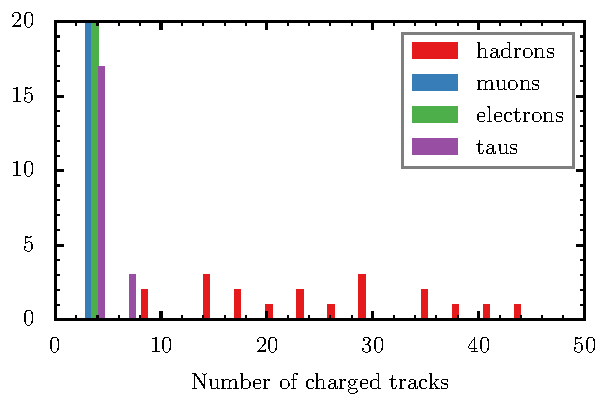
\includegraphics[width=1.0\textwidth]{./talkfigs/pdf/Ctrk(N).pdf}\\
			\begin{itemize}
				\item Separate hadrons and charged leptons
				\item \textbf{$e, \mu$} number of tracks $<5$
				\item $\tau$ number of tracks $<6$
				\item hadrons number of tracks $>7$
			\end{itemize}
		\column[c]{0.5\textwidth}
			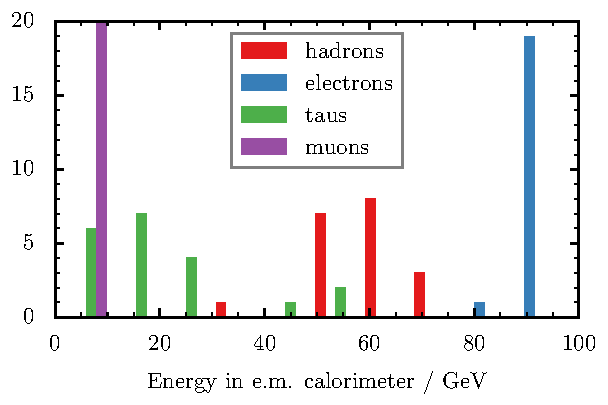
\includegraphics[width=1.0\textwidth]{./talkfigs/pdf/Ecal(SumE).pdf}
			\begin{itemize}
				\item Separate electrons, muons
				\item $\mu$ less than \SI{8}{GeV}
				\item $e$ minimum \SI{60}{GeV}
				\vspace{2.8em}
			\end{itemize}
	\end{columns}
\end{frame}

\begin{frame}{Preliminary Cut Selections}
	\begin{center}
		\begin{tabular}{lcccc}
			\toprule
			&\multicolumn{4}{c}{selected channel}  \\ \cmidrule(r){2-5}
			& electrons & muons & tauons & hadrons \\
			\midrule
			total momentum / \si{GeV} & $> 30$ & $> 65$ & $< 65$ & --\\
			number charged tracks & $< 5$  & $< 5$  & $< 6$ & $>7$ \\
			e.m. cal. energy / \si{GeV}  & $> 60$ & $< 8$ & $< 60$ & -- \\
			had. cal. energy / \si{GeV}  & $< 2$  & $< 10$ & -- & -- \\
			\bottomrule
		\end{tabular}
	\end{center}
	\begin{itemize}
		\item Test sample with events from unknown decay channels
		\item Apply cuts on events and check by eye
		\item All but one event from test sample identified correctly
		\item Problem: only few events, need more statistics to make more precise cuts
	\end{itemize}
\end{frame}

\section{Part II: Statistical Analysis of $\mathrm{Z}^0$ Decays}
\begin{frame}{Part II: Statistical Analysis of $\mathrm{Z}^0$ Decays}
	\begin{itemize}
		\setlength\itemsep{2.em}
		\item Analysis of data gathered by OPAL at LEP
		\begin{itemize}
			\setlength\itemsep{0.5em}
			\item event displays unfeasible ($\sim \num{400000}$ events)
			\item data analysis software \texttt{PAW} used instead
		\end{itemize}
		
		\item Determination of
		\begin{itemize}
			\setlength\itemsep{0.5em}
			\item cross sections $\sigma_f$
			
			\item mass $M_\mathrm{Z}$ and total decay-width $\Gamma_\mathrm{Z}$
			
			\item partial decay-widths $\Gamma_f$ (lepton universality, number of light neutrino generations $N_\nu$)
			
			\item electroweak mixing $\sin^2\theta_\mathrm{W}$ (forward-backward asymmetry)
		\end{itemize}
	\end{itemize}
\end{frame}

\begin{frame}{Part II: Statistical Analysis of $\mathrm{Z}^0$ Decays}
	\textbf{Procedure:}
	\begin{enumerate}
		\setlength\itemsep{2.em}
		\item Preparation of the measurement (MC-data)
		\begin{itemize}
			\setlength\itemsep{0.5em}
			\item refine selection cuts for the different decay-channels
			
			\item separate $s$- and $t$-channel in $\mathrm{e}^+ + \mathrm{e}^- \rightarrow \mathrm{e}^+ + \mathrm{e}^-$
			
			\item determine the efficiency of the applied cuts
		\end{itemize}
		
		\item Analysis of OPAL data (exp.\ data)
		\begin{itemize}
			\setlength\itemsep{0.5em}
			\item separate the decay-channels with the selection cuts
			
			\item efficiency formalism to obtain the total number of events
			
			\item calculation of the physical quantities
		\end{itemize}
	\end{enumerate}
\end{frame}

\subsection{Analysis of Monte-Carlo Data}

\begin{frame}{Analysis of Monte-Carlo Data}
	\begin{itemize}
		\setlength\itemsep{2.em}
		\item Simulated events with detector response separated into decay channels $\mathrm{e}, \mu, \tau, \mathrm{q}$ (\num{100000} events each)
	\end{itemize}
	\begin{columns}
		\column[c]{0.6\textwidth}
			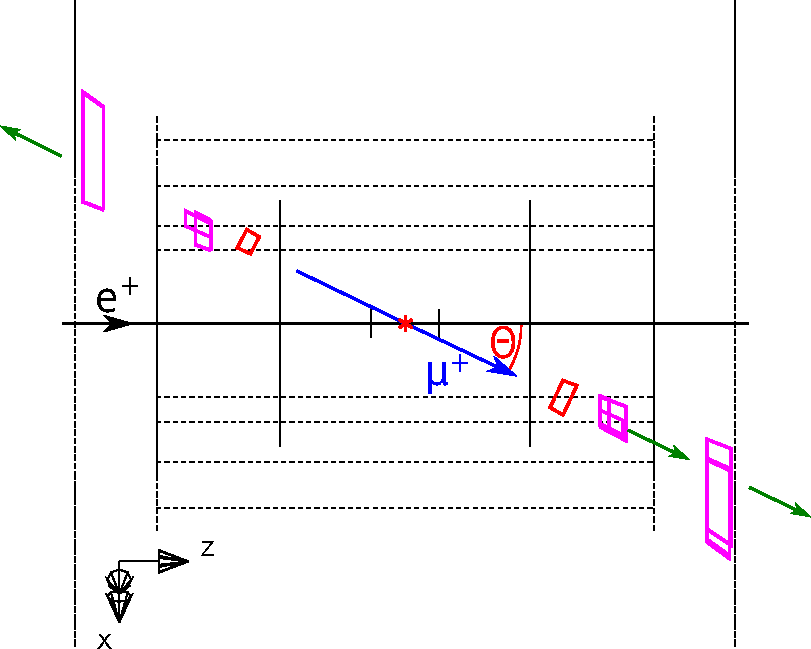
\includegraphics[width=\textwidth]{./talkfigs/pdf/mm_05_side.pdf}
		
		\column[c]{0.4\textwidth}
			Detector variables for each event:
			\begin{itemize}
				\setlength{\itemsep}{0.5em}
				\item \texttt{ncharged}
				\item \texttt{pcharged}
				\item \texttt{e\_ecal}
				\item \texttt{e\_hcal}
				\item \texttt{cos\_thet}
			\end{itemize}
	\end{columns}
\end{frame}

\begin{frame}{Refining the Cuts -- \texttt{pcharged}}
	\begin{center}
		\begin{overpic}[height=0.9\textheight, trim=0 0 0 20, clip]{./talkfigs/pdf/pcharged_uncut.pdf}
			\put(31.3,86.7){\fcolorbox{black}{white}{\makebox(12,3)[c]{\footnotesize electrons}}}
			\put(78.8,86.7){\fcolorbox{black}{white}{\makebox(12,3)[c]{\footnotesize muons}}}
			\put(31.3,39.3){\fcolorbox{black}{white}{\makebox(12,3)[c]{\footnotesize taus}}}
			\put(78.8,39.3){\fcolorbox{black}{white}{\makebox(12,3)[c]{\footnotesize hadrons}}}
		\end{overpic}
	\end{center}
\end{frame}

\begin{frame}[noframenumbering]{Refining the Cuts -- \texttt{pcharged}}
	\begin{center}
		\begin{overpic}[height=0.9\textheight, trim=0 0 0 20, clip]{./talkfigs/pdf/pcharged_coscut.pdf}
			\put(31.3,86.7){\fcolorbox{black}{white}{\makebox(12,3)[c]{\footnotesize electrons}}}
			\put(78.8,86.7){\fcolorbox{black}{white}{\makebox(12,3)[c]{\footnotesize muons}}}
			\put(31.3,39.3){\fcolorbox{black}{white}{\makebox(12,3)[c]{\footnotesize taus}}}
			\put(78.8,39.3){\fcolorbox{black}{white}{\makebox(12,3)[c]{\footnotesize hadrons}}}
		\end{overpic}
	\end{center}
\end{frame}

\begin{frame}<1>[label=cutsummary]{Refining the Cuts -- Summary}
	\begin{itemize}
		\item<1-> electrons and muons: $\left| \cos\theta \right| < 0.9$ (unreconstructible events)
		\item<6-> electrons: $\cos\theta < 0.5$ ($s$-channel)
	\end{itemize}
	\vfill
	\pause
	\begin{center}
		\begin{tabular}{lcccc}
			\toprule
			&\multicolumn{4}{c}{selected channel}  \\ \cmidrule(r){2-5}
			& electrons & muons & tauons & hadrons \\
			\midrule
			\texttt{pcharged} & \only<2->{$> 30$} & \only<2->{$> 55$} & \only<2->{$>1\,\land\,<75$} & \only<2->{--}\\
			\texttt{ncharged} & \only<3->{$< 5$}  & \only<3->{$< 4$}  & \only<3->{$< 8$} & \only<3->{$\geq 8$} \\
			\texttt{e\_ecal}  & \only<4->{$> 70$} & \only<4->{$< 15$}  & \only<4->{$< 75$} & \only<4->{$> 20$} \\
			\texttt{e\_hcal}  & \only<5->{$< 15$}  & \only<5->{$< 25$} & \only<5->{--} & \only<5->{--} \\
			\bottomrule
		\end{tabular}
	\end{center}
\end{frame}

\begin{frame}{Refining the Cuts -- \texttt{pcharged}}
	\begin{center}
		\begin{overpic}[height=0.9\textheight, trim=0 0 0 20, clip]{./talkfigs/pdf/pcharged_cuts.pdf}
			\put(31.3,86.7){\fcolorbox{black}{white}{\makebox(12,3)[c]{\footnotesize electrons}}}
			\put(78.8,86.7){\fcolorbox{black}{white}{\makebox(12,3)[c]{\footnotesize muons}}}
			\put(31.3,39.3){\fcolorbox{black}{white}{\makebox(12,3)[c]{\footnotesize taus}}}
			\put(78.8,39.3){\fcolorbox{black}{white}{\makebox(12,3)[c]{\footnotesize hadrons}}}
		\end{overpic}
	\end{center}
\end{frame}

\againframe<2>{cutsummary}


\begin{frame}{Refining the Cuts -- \texttt{ncharged}}
	\begin{center}
		\begin{overpic}[height=0.9\textheight, trim=0 0 0 20, clip]{./talkfigs/pdf/ncharged_cuts.pdf}
			\put(31.3,86.7){\fcolorbox{black}{white}{\makebox(12,3)[c]{\footnotesize electrons}}}
			\put(78.8,86.7){\fcolorbox{black}{white}{\makebox(12,3)[c]{\footnotesize muons}}}
			\put(31.3,39.3){\fcolorbox{black}{white}{\makebox(12,3)[c]{\footnotesize taus}}}
			\put(78.8,39.3){\fcolorbox{black}{white}{\makebox(12,3)[c]{\footnotesize hadrons}}}
		\end{overpic}
	\end{center}
\end{frame}

\againframe<3>{cutsummary}

\begin{frame}{Refining the Cuts -- \texttt{e\_ecal}}
	\begin{center}
		\begin{overpic}[height=0.9\textheight, trim=0 0 0 20, clip]{./talkfigs/pdf/e_ecal_cuts.pdf}
			\put(31.3,86.7){\fcolorbox{black}{white}{\makebox(12,3)[c]{\footnotesize electrons}}}
			\put(78.8,86.7){\fcolorbox{black}{white}{\makebox(12,3)[c]{\footnotesize muons}}}
			\put(31.3,39.3){\fcolorbox{black}{white}{\makebox(12,3)[c]{\footnotesize taus}}}
			\put(78.8,39.3){\fcolorbox{black}{white}{\makebox(12,3)[c]{\footnotesize hadrons}}}
		\end{overpic}
	\end{center}
\end{frame}

\againframe<4>{cutsummary}

\begin{frame}{Refining the Cuts -- \texttt{e\_hcal}}
	\begin{center}
		\begin{overpic}[height=0.9\textheight, trim=0 0 0 20, clip]{./talkfigs/pdf/e_hcal_cuts.pdf}
			\put(31.3,86.7){\fcolorbox{black}{white}{\makebox(12,3)[c]{\footnotesize electrons}}}
			\put(78.8,86.7){\fcolorbox{black}{white}{\makebox(12,3)[c]{\footnotesize muons}}}
			\put(31.3,39.3){\fcolorbox{black}{white}{\makebox(12,3)[c]{\footnotesize taus}}}
			\put(78.8,39.3){\fcolorbox{black}{white}{\makebox(12,3)[c]{\footnotesize hadrons}}}
		\end{overpic}
	\end{center}
\end{frame}

\againframe<5>{cutsummary}

\begin{frame}{Separating $s$- and $t$-Channel in $\mathrm{e}^+ + \mathrm{e}^- \rightarrow \mathrm{e}^+ + \mathrm{e}^-$}
	\begin{columns}
		\column[c]{0.5\textwidth}
			\begin{itemize}
				\setlength\itemsep{2.em}
				\item<2-> $t$-channel dominant at small scattering angles
				
				\item<3-> remove most $t$-channel events by cutting $\cos\theta < 0.5$
				
				\item<4-> correction for the number of $s$-channel events
				\begin{align*}
					\kappa &= \frac{\int_{-1}^{1} (1 + \cos^2\theta) \, \mathrm{d}\cos\theta}{\int_{-0.9}^{0.5} (1 + \cos^2\theta) \, \mathrm{d}\cos\theta} \\
					&\approx  1.5829
				\end{align*}
			\end{itemize}
		\column[c]{0.5\textwidth}
			\includegraphics<1>[width=1.0\textwidth]{./talkfigs/pdf/cos_thet_uncut.pdf}
			\includegraphics<2>[width=1.0\textwidth]{./talkfigs/pdf/cos_thet_annotated.pdf}
			\includegraphics<3->[width=1.0\textwidth]{./talkfigs/pdf/cos_thet_cuts.pdf}
	\end{columns}
\end{frame}

\againframe<6>{cutsummary}

\begin{frame}{Efficiency Matrix}
	Using the chosen cuts quantify the:
	\begin{itemize}
		\setlength\itemsep{1.em}
		\item fraction of correctly identified events
		\item probability of misidentifying an event
	\end{itemize}
	\vspace{0.7cm}
	\pause
	Matrix formalism:
	\begin{itemize}
		\setlength\itemsep{1.em}
		\item number of events in different channels separated in vectors
		\begin{align*}
			&\vec{n} = \begin{pmatrix}
			\alert{n_\mathrm{e,s}} & n_\mathrm{\mu} & n_\mathrm{\tau} & n_\mathrm{q}
			\end{pmatrix}^\mathrm{T}
			\qquad
			&\vec{N} = \begin{pmatrix}
			\alert{N_\mathrm{e,s}} & N_\mathrm{\mu} & N_\mathrm{\tau} & N_\mathrm{q}
			\end{pmatrix}^\mathrm{T}
		\end{align*}
		$\vec{n}$: number of events after cuts\qquad $\vec{N}$: total number of events 
		
		\item efficiency matrix definition
		\begin{align*}
			\vec{n} = E \cdot \vec{N}
		\end{align*}
		
		
	\end{itemize}
\end{frame}


\begin{frame}{Efficiency Matrix}
	Apply cuts to Monte-Carlo datasets:
	\begin{center}
		\begin{tabular}{rS[table-format=6.0]S[table-format=6.0]S[table-format=6.0]S[table-format=6.0]}
	\toprule
	&\multicolumn{4}{c}{dataset}  \\ \cmidrule(r){2-5}
	$j$ & {$\mathrm{e}$} & {$\mathrm{\mu}$} & {$\mathrm{\tau}$} & {$\mathrm{q}$}\\
	\midrule
	total & 100000 & 100000 & 100000 & 100000\\
	precut & 93454 & 93979 & 79051 & 97848\\
	$n_{\mathrm{e}j}$ & 20229 & 0 & 692 & 6 \\
	$n_{\mathrm{\mu}j}$ & 1 & 78537 & 4089 & 0 \\
	$n_{\mathrm{\tau}j}$ & 117 & 549 & 76651 & 503 \\
	$n_{\mathrm{q}j}$ & 0 & 0 & 934 & 97533 \\
 	\bottomrule
\end{tabular}
	\end{center}
	\vspace{0.4cm}
	\pause
	Calculate matrix elements:
	\begin{align*}
		E_{ij} = \frac{n_{ij}}{N_j} \qquad\qquad N_\mathrm{e,s} = n_\mathrm{ee} \cdot \underbrace{\frac{100000}{93454}}_{\substack{\text{precut}\\\text{efficiency}}} \cdot \underbrace{\kappa}_{\substack{\text{correct.} \\ \text{due to} \\ \text{ang.\ cut}}} = 34136
	\end{align*}
\end{frame}


\begin{frame}{Efficiency Matrix}
	Efficiency matrix for our cuts:
	\begin{align*}
	\footnotesize
	E = \begin{pmatrix*}[r]
	59.259 & 0.001 & 0.117 & 0.000 \\
	0.000 & 78.537 & 0.549 & 0.000 \\
	2.027 & 4.089 & 76.651 & 0.934 \\
	0.018 & 0.000 & 0.503 & 97.533 \\
	\end{pmatrix*} \times 10^{-2}
	\end{align*}
	
	With errors from binomial statistics:
	\begin{align*}
	\footnotesize
	\Delta E = \begin{pmatrix*}[r]
	0.266 & 0.000 & 0.000 & 0.000 \\
	0.000 & 0.130 & 0.024 & 0.000 \\
	0.077 & 0.063 & 0.134 & 0.031 \\
	0.008 & 0.000 & 0.023 & 0.050 \\
	\end{pmatrix*} \times 10^{-2}
	\end{align*}
	
	\pause
	
	\vspace{0.5cm}
	
	\textbf{Problem:} Experimentally only $\vec{n}$ is measured. Invert the efficiency matrix.
	\begin{align*}
		\vec{N} = E^{-1} \cdot \vec{n}
	\end{align*}
\end{frame}

\begin{frame}{Efficiency Matrix}
	Numerical inversion:
	\begin{align*}
	\footnotesize
	E^{-1} = \begin{pmatrix*}[r]
	168.758 & 0.011 &-0.258 & 0.002 \\
	0.312 & 127.376 &-0.912 & 0.009 \\
	-4.465 &-6.796 & 130.525 &-1.250 \\
	-0.007 & 0.035 &-0.673 & 102.536 \\
	\end{pmatrix*} \times 10^{-2}
	\end{align*}
	
	\vfill
	
	Errors by Monte-Carlo error propagation (\num{100000} samples):
	\begin{align*}
	\footnotesize
	\Delta E^{-1} = \begin{pmatrix}
	0.756 & 0.001 & 0.002 & 0.001 \\
	0.002 & 0.211 & 0.039 & 0.001 \\
	0.170 & 0.105 & 0.227 & 0.041 \\
	0.013 & 0.002 & 0.030 & 0.052 \\
	\end{pmatrix} \times 10^{-2}
	\end{align*}
\end{frame}

\subsection{Analysis of OPAL Data}

\begin{frame}{Analysis of OPAL Data}
	\begin{itemize}
		\setlength\itemsep{1.5em}
		\item total number of events $\vec{N}$ now unknown
		\begin{itemize}
			\setlength\itemsep{.5em}
			\item apply cuts to experimental data to get $\vec{n}$
			\item determine $\vec{N}$ using:\quad $\vec{N} = E^{-1} \cdot \vec{n}$
		\end{itemize}
		
		\pause
		
		\item determine cross section $\sigma_i$ as a function of cm.\ energy
		\begin{itemize}
			\setlength\itemsep{.5em}
			\item data contains events at multiple \texttt{e\_lep} -- select energies using cuts
			\item after identifying the channels calculate cross section
			\begin{align*}
				\sigma_i = \frac{N_i}{\int \mathcal{L} \, \mathrm{d}t} + \underbrace{\mathrm{corr}_i(\sqrt{s})}_{\substack{\text{radiation} \\ \text{correction}}} \qquad i \in \left\{ \mathrm{e}, \mathrm{\mu}, \mathrm{\tau}, \mathrm{q} \right\}
			\end{align*}
			with integrated luminosity $\int \mathcal{L} \, \mathrm{d}t$ at a given energy
		\end{itemize}
	\end{itemize}
\end{frame}

\begin{frame}{Cross Section \& Breit-Wigner Fit}
	\begin{itemize}
		\setlength\itemsep{1.5em}
		
		\item for each channel fit a Breit-Wigner resonance
			\begin{align*}
			\sigma(E_\mathrm{cm}; A, M_\mathrm{Z}, \Gamma_\mathrm{Z}) = \frac{A}{2\pi} \frac{\Gamma_\mathrm{Z}}{\left( E_\mathrm{cm} - M_\mathrm{Z} \right)^2 + \Gamma_\mathrm{Z}^2 / 4}
			\end{align*}
			
			\begin{itemize}
				\setlength\itemsep{.5em}
				\item mass $M_\mathrm{Z}$
				\item total decay width $\Gamma_\mathrm{Z}$
				\item factor $A$ proportional to the cross section at peak
				\begin{align*}
					\sigma_\mathrm{peak} = \frac{2A}{\pi \Gamma_\mathrm{Z}}
				\end{align*}
			\end{itemize}
		
	\end{itemize}
\end{frame}

\begin{frame}{Cross Section \& Breit-Wigner Fit}
	\centering
	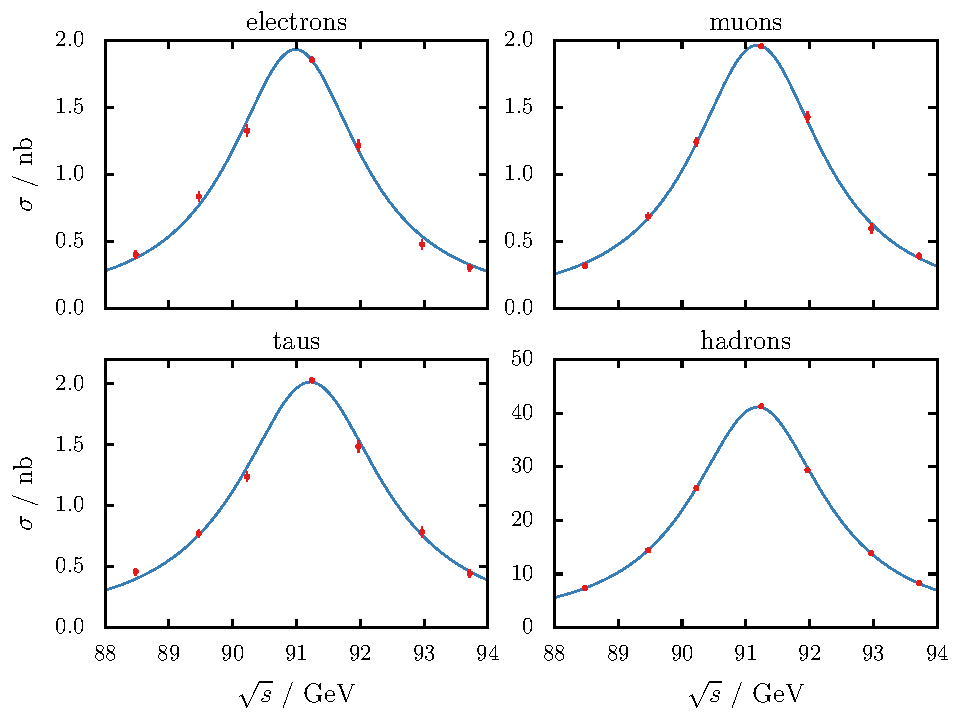
\includegraphics[height=0.9\textheight]{./talkfigs/pdf/cross_sections.pdf}
\end{frame}

\begin{frame}{Cross Section \& Breit-Wigner Fit}
	\begin{center}
		\begin{tabular}{lS[table-format=2.2,table-figures-uncertainty=3]S[table-format=1.2,table-figures-uncertainty=3]S[table-format=2.3,table-figures-uncertainty=4]S[table-format=1.3]}
	\toprule
	{}& {$M_\mathrm{Z}$ / GeV} & {$\Gamma_\mathrm{Z}$ / GeV} & {$\sigma^\mathrm{peak}$ / nb} & {$\chi_\mathrm{red}^2$} \\
	\midrule
	electrons & 90.99 +- 0.24 & 2.47 +- 0.11 & 1.934 +- 0.077 & 2.796 \\
	muons & 91.18 +- 0.12 & 2.47 +- 0.05 & 1.966 +- 0.033 & 0.847 \\
	tauons & 91.22 +- 0.26 & 2.72 +- 0.10 & 2.015 +- 0.069 & 2.451 \\
	hadrons & 91.19 +- 0.70 & 2.53 +- 0.02 & 41.138 +- 0.270 & 1.776 \\	
	\midrule
	mean & 91.15 +- 0.10 & 2.52 +- 0.02 & {--} & {--} \\
	\bottomrule	
\end{tabular}
	\end{center}
	\vfill
	\pause
	Error weighted means:
	\begin{alignat*}{2}
		&M_\mathrm{Z} = \SI{91.15 +- 0.1}{GeV} \qquad &&M_\mathrm{Z}^\mathrm{Lit.} = \SI{91.1876 +- 0.0021}{GeV}\\[0.5em]
		&\Gamma_\mathrm{Z} = \SI{2.52 +- 0.02}{GeV} \qquad &&\Gamma_\mathrm{Z}^\mathrm{Lit.} = \SI{2.4952 +- 0.0023}{GeV}
	\end{alignat*}
	lit.\ values from \cite{pdg}
\end{frame}

\begin{frame}{Partial Decay Widths}
	\begin{itemize}
		\item cross section at resonance from theory
			\begin{align*}
			\sigma_f^\mathrm{peak} = \frac{12 \pi}{M_\mathrm{Z}^2} \cdot \frac{\alert{\Gamma_\mathrm{e}}}{\Gamma_\mathrm{Z}} \cdot \frac{\Gamma_f}{\Gamma_\mathrm{Z}} \qquad f \in \left\{ \mathrm{e}, \mathrm{\mu}, \mathrm{\tau}, \mathrm{q} \right\}
			\end{align*}
		
		\begin{enumerate}
			\item<2-> calculate $\Gamma_\mathrm{e}$
				 \begin{align*}
				 	\Gamma_\mathrm{e} = \sqrt{\frac{M_\mathrm{Z}^2}{12 \pi} \, \Gamma_\mathrm{Z}^2 \sigma_\mathrm{e}^\mathrm{peak}}
				 \end{align*}
				 
			\item<3-> use $\Gamma_\mathrm{e}$ to determine $\Gamma_f$ for $f \in \left\{ \mathrm{\mu}, \mathrm{\tau}, \mathrm{q} \right\}$
				\begin{align*}
					\Gamma_f = \frac{M_\mathrm{Z}^2}{12 \pi } \, \frac{\Gamma_\mathrm{Z}^2 }{\Gamma_\mathrm{e}} \sigma_f^\mathrm{peak}
				\end{align*}
		\end{enumerate}
	\end{itemize}	
\end{frame}

\begin{frame}{Partial Decay Widths}
	\begin{itemize}
		\setlength\itemsep{2em}
		\item resulting partial decay widths
			\begin{alignat*}{2}
			&\Gamma_\mathrm{e} = \SI{83.6 +- 1.8}{MeV} \qquad
			&&\Gamma_\mathrm{\mu} = \SI{85.0 +- 2.3}{MeV}\\
			&\Gamma_\mathrm{\tau} = \SI{87.1 +- 3.5}{MeV}\qquad
			&&\Gamma_\mathrm{hadrons} = \SI{1778.5 +- 39}{MeV}
			\end{alignat*}
		
		\item<2-> literature values \cite{pdg}
		\begin{alignat*}{2}
		&\Gamma_\ell = \SI{83.984 +- 0.086}{MeV} \qquad
		&&\Gamma_\mathrm{hadrons} = \SI{1744.4 +- 2.0}{MeV}
		\end{alignat*}
		
		\item<3-> consistent with lepton universality
			\begin{align*}
				&\frac{\Gamma_\mathrm{\mu}}{\Gamma_\mathrm{e}} = \num{1.017 +- 0.044} \qquad 
				&\frac{\Gamma_\mathrm{\tau}}{\Gamma_\mathrm{e}} = \num{1.042 +- 0.055}
			\end{align*}
	\end{itemize}
\end{frame}

\begin{frame}{Number of Light Neutrino Generations}
	\begin{itemize}
		\setlength\itemsep{2em}
		\item<1-> full decay width of the Z-boson
		\begin{align*}
			\Gamma_\mathrm{Z} = \Gamma_\mathrm{e} + \Gamma_\mathrm{\mu} + \Gamma_\mathrm{\tau} + N_\nu \Gamma_\nu + \Gamma_\mathrm{hadrons}
		\end{align*}
		with $N_\nu$ number of neutrino generations $M_\nu < M_\mathrm{Z} / 2$
		
		\item<2-> $\Gamma_\nu$ known from theory: \quad $\Gamma_\nu = \SI{167.6}{MeV}$ \quad \cite{instructions}
		
		\item<3-> number of light neutrino generations
			\begin{align*}
			N_\nu &= \frac{\Gamma_\mathrm{Z} - \Gamma_\mathrm{e} - \Gamma_\mathrm{\mu} - \Gamma_\mathrm{\tau} - \Gamma_\mathrm{hadrons}}{\Gamma_\nu} \\[1.0em]
			&= \num{2.94 +- 0.24} \quad \text{(using measured values)}
			\end{align*}
	\end{itemize}
\end{frame}

\begin{frame}{Forward-Backward Asymmetry}
	\begin{itemize}
		\setlength\itemsep{1.5em}
		\item<1-> asymmetric number of events in forward- and backward-hemisphere
		\begin{align*}
			\cos\theta > 0~\text{(forward)} \qquad \cos\theta < 0~\text{(backward)}
		\end{align*}
		
		\item<2-> observable in all leptonic decay channels -- clearest signature for muons
		
		
		\item<3-> forward-backward asymmetry
			\begin{align*}
				A_\mathrm{FB} = \frac{n_\mathrm{F} - n_\mathrm{B}}{n_\mathrm{F} + n_\mathrm{B}} + \underbrace{\mathrm{corr}(\sqrt{s})}_{\substack{\text{radiation} \\ \text{correction}}}
			\end{align*}
			function of cm.\ energy
	\end{itemize}
\end{frame}

\begin{frame}{Forward-Backward Asymmetry}
	\begin{columns}
		\column[c]{0.45\textwidth}
		\begin{itemize}
			\setlength\itemsep{1.5em}
			\item<2-> asymmetry at peak of resonance
			\begin{align*}
				A_\mathrm{FB}^\mathrm{peak} \approx 3\left( 1 - 4 \sin^2\theta_\mathrm{W} \right)
			\end{align*}
			
			\item<3-> approx.\ peak asymmetry with measurement at $\sqrt{s} = \SI{91.24}{GeV}$
			\begin{align*}
			A_\mathrm{FB}^\mathrm{peak} \approx \num{0.0119 +- 0.0075}
			\end{align*}
		\end{itemize}
		\column[c]{0.55\textwidth}
			\begin{center}
				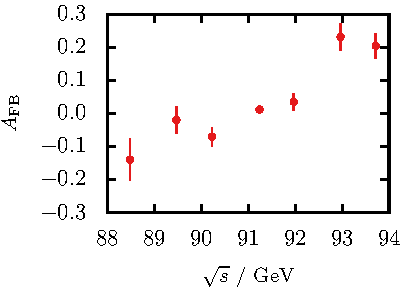
\includegraphics{./talkfigs/pdf/afb.pdf}
			\end{center}
	\end{columns}

\end{frame}

\begin{frame}{Forward-Backward Asymmetry}
		\begin{itemize}
			\setlength\itemsep{1.5em}
			\item calculate electroweak mixing
			\begin{align*}
			\sin^2\theta_\mathrm{W} &= \frac{1}{4} \left( 1 - \sqrt{A_\mathrm{FB}^\mathrm{peak} / 3} \right) \\[0.1em]
			&= \num{0.234 +- 0.005}
			\end{align*}
			
			\item<2-> good agreement with literature value \cite{pdg}
			\begin{align*}
				\sin^2\theta_\mathrm{W} = \num{0.23126 +- 0.00005}
			\end{align*}
			
			
		\end{itemize}
\end{frame}




\section{Conclusion}

\begin{frame}
	\begin{center}
		\LARGE
		\textbf{Thank you for your attention!}
	\end{center}
\end{frame}

\begin{frame}{Bibliography}
	\scriptsize
	\begin{thebibliography}{9}
		\bibitem[Instructions]{instructions}
			\emph{Instructions for E213: Analysis of $Z^0$ decays},
			Universität Bonn.
		
		\bibitem[PDG]{pdg}
			K.A. Olive \textit{et al.} (Particle Data Group),
			\emph{The Review of Particle Physics},
			Chin.\ Phys.\ C, \textbf{38}, 090001 (2014) and 2015 update.
	\end{thebibliography}
\end{frame}

\beginbackup

\begin{frame}{Error-Estimates from the Binomial Distribution}
	\begin{align*}
		\Delta n_i = \sqrt{N \cdot \left[ \frac{n_i}{N} - \left( \frac{n_i}{N} \right)^2 \right]}
	\end{align*}
\end{frame}

\backupend

\end{document}